\section {Game 1}

\subsection {Brief Description}

The objective of this game is to return as many tokens as possible to the designated team area. Gameplay terminates after a lapsed period of time.

\subsection {Details}

\begin {itemize}
\item {Each round will contain 4 teams.}
\item {20 tokens will be placed in the arena prior to the commencement of the round.}
\item {Each team will be designated a zone.}
\item {All tokens will be the same colour.}
\item {Gameplay commences at the sound of the alarm.}
\item {Gameplay will terminate the second time the alarm sounds.}
\item {Gameplay will end after 5 minutes or when no tokens remain in the arena.}\item {Each token placed in a team's zone at the end of the round will contribute 10 points to a team's competition score}
\end {itemize}

\subsection {Rules}

\begin {itemize}
\item Teams are designated one zone only.
\item Tokens placed in the wrong zone will count towards the token count of the team that owns that particular zone.
\item Tokens in robot possession at the end of gameplay will not contribute towards the team's score for that game.
\end {itemize}

\clearpage
\newpage

\subsection {Arena Layout}

\begin {figure}[h]
\begin {center}
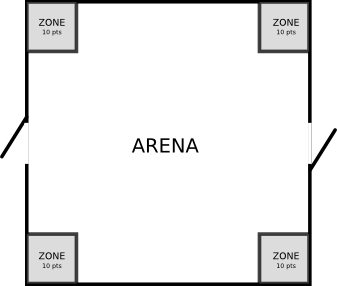
\includegraphics[keepaspectratio, scale =1]{../arena/arenagame1.png}
\caption{\small{\emph{The General Arena Layout}}}
\label {fig:arena}
\end {center}
\end {figure}
